\documentclass[12pt]{article}
\usepackage{amsmath, amssymb}
\usepackage{graphicx}
\usepackage{listings}
\usepackage{xcolor}
\usepackage{geometry}
\geometry{a4paper, margin=1in}

\title{Binomial Distribution Analysis of 100 Coin Tosses}
\author{Sarvesh Adithya J}
\date{July 25, 2025}

\definecolor{codegray}{gray}{0.95}
\lstset{
  backgroundcolor=\color{codegray},
  basicstyle=\ttfamily\small,
  frame=single,
  breaklines=true,
  postbreak=\mbox{\textcolor{red}{$\hookrightarrow$}\space},
  showstringspaces=false,
}

\begin{document}

\maketitle

\begin{abstract}
This project explores the Binomial distribution in the context of 100 fair coin tosses. Using Python's \texttt{scipy.stats} and \texttt{matplotlib}, the Probability Mass Function (PMF) and Cumulative Distribution Function (CDF) are calculated and visualized. This demonstrates the behavior of a large number of binary trials and highlights how the Binomial distribution approximates a normal curve as the number of trials increases.
\end{abstract}

\section{Introduction}
The Binomial distribution is a discrete probability distribution that describes the number of successes in a fixed number of independent Bernoulli trials. In this experiment, we simulate the tossing of a fair coin 100 times and analyze the distribution of the number of heads.

\section{Objective}
To compute and visualize:
\begin{itemize}
    \item The Probability Mass Function (PMF)
    \item The Cumulative Distribution Function (CDF)
\end{itemize}
for the Binomial distribution with $n = 100$ trials and $p = 0.5$ probability of success.

\section{Methodology}
We used the Python programming language with the following libraries:
\begin{itemize}
    \item \texttt{numpy}: for array manipulations
    \item \texttt{matplotlib.pyplot}: for plotting PMF and CDF
    \item \texttt{scipy.stats.binom}: for computing PMF and CDF
\end{itemize}

\section{Python Code}
Below is the Python code used to compute and plot the PMF and CDF:

\begin{lstlisting}[language=Python]
import numpy as np
import matplotlib.pyplot as plt
from scipy.stats import binom

n = 100
p = 0.5

x = np.arange(0, n + 1)
pmf_values = binom.pmf(x, n, p)
cdf_values = binom.cdf(x, n, p)

plt.figure(figsize=(12, 5))

plt.subplot(1, 2, 1)
plt.stem(x, pmf_values, basefmt=" ")
plt.title('PMF of 100 Coin Tosses')
plt.xlabel('Number of Heads')
plt.ylabel('Probability')

plt.subplot(1, 2, 2)
plt.plot(x, cdf_values, 'b-')
plt.title('CDF of 100 Coin Tosses')
plt.xlabel('Number of Heads')
plt.ylabel('Cumulative Probability')

plt.tight_layout()
plt.show()
\end{lstlisting}

\section{Results}
The resulting plots clearly demonstrate the Binomial distribution's characteristics:
\begin{itemize}
    \item The PMF peaks around 50 heads, showing the most probable outcome.
    \item The CDF increases gradually and approaches 1 as the number of heads approaches 100.
\end{itemize}

\begin{figure}[h]
\centering
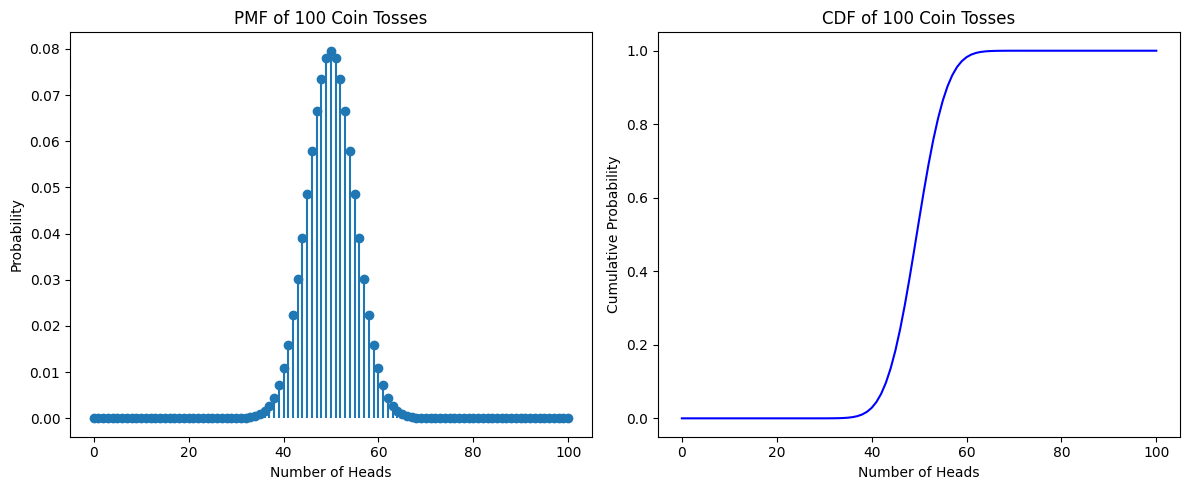
\includegraphics[width=0.9\textwidth]{cdf_pmf_plot.png}
\caption{PMF and CDF of 100 Coin Tosses}
\end{figure}

\section{Conclusion}
This experiment successfully visualized the behavior of a large Binomial distribution using Python. As expected, the PMF is symmetric and centered around 50, while the CDF rises steeply in that region. This experiment validates the theoretical understanding of the Binomial distribution and its real-world simulation through code.

\end{document}
